\documentclass[UTF8]{ctexart}
\usepackage{amsmath,graphicx,tikz,caption,subfigure}
\usepackage[algo2e,ruled,vlined]{algorithm2e}
\usepackage{stfloats}
\usepackage{float}
\usepackage[a4paper]{geometry}
\geometry{left=0.5cm,right=0.5cm,top=0.5cm,bottom=0.5cm}
\title{\textbf{Report2}}
\author{胡琦浩  PB21000235}
\date{\today}

\begin{document}
\maketitle
\section{问题}
用16807产生器测试随机数序列中满足关系$X_{n-1}>X_{n+1}>X_n$的比重,讨论Fibonacci延迟产生器中出现这种关系的比重

\section{方法}
\subsection{16807产生器}
读取第一题生成的随机数csv文件,并储存到列表中,用for循环遍历整个列表寻找满足此关系的n值,最后统计满足条件n的数量

\subsection{Fibonacci产生器}
采用带减法的产生器:
\begin{equation}
    I_n=I_{n-22}-I_{n-43}-C
\end{equation}
\begin{equation}
    \begin{cases}
        C=0  & I_n\mbox{>=  0} \\
        C=1,\quad I_n=I_n+(2^{32}-5) & I_n\mbox{<0}
    \end{cases}
\end{equation}
在此方法中,我们要先得到前43个随机数,故用到第一题生成的前43个I值

\section{实验结果}
\begin{figure}[htbp]
    \centering
    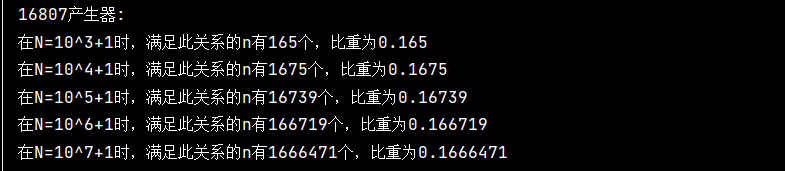
\includegraphics[scale=0.5]{1}
    \caption{16807产生器}
\end{figure}
\begin{figure}[htbp]
    \centering
    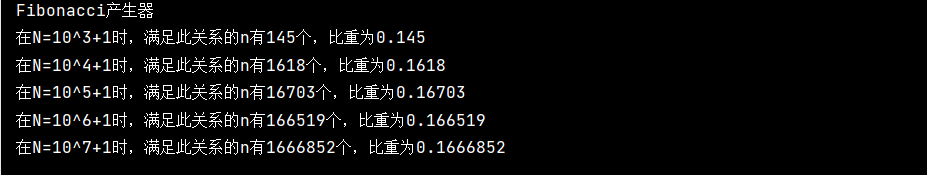
\includegraphics[scale=0.5]{2}
    \caption{Fibonacci产生器}
\end{figure}
由图中结论可看出两随机数产生器在N足够大时,结果均趋向于理想值:$\frac{1}{6}$.因此两随机数产生器产生的随机数都很好

\section{总结}
通过完成本题,发现两种随机数产生器都可以产生很好的随机数,均匀性很好
\end{document}